\begin{figure}[t]
\begin{center}
	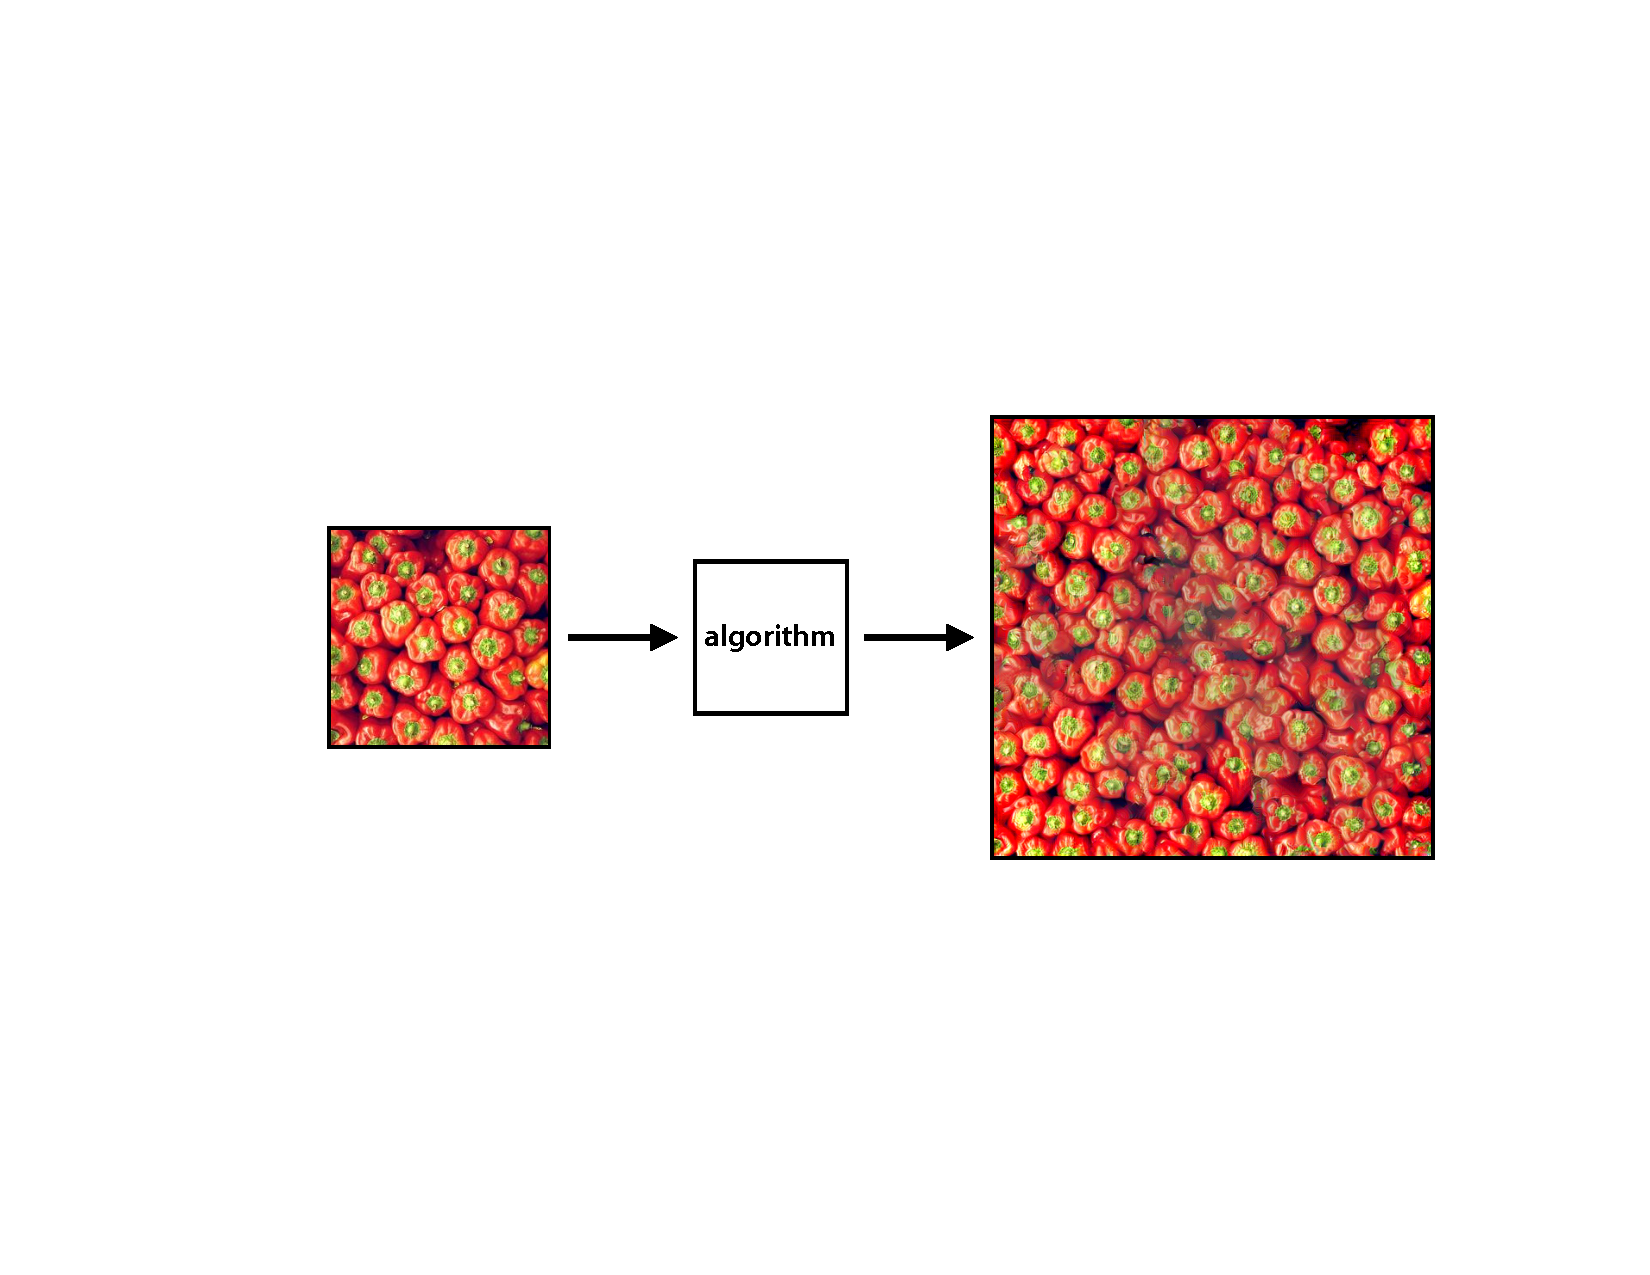
\epsfig{file=texture_synthesis.pdf, width = 0.8\textwidth}\\
	\caption[Texture synthesis]{(Static) texture synthesis is the process of algorithmically constructing a texture (right) that matches or extends a given source texture (left) by taking advantage of its structural content.}
	\vspace{-0.65cm}
	\label{fig:texture_synthesis}
\end{center}
\end{figure}